\documentclass{report}
\usepackage{titletoc}
\usepackage{graphicx}
\usepackage{amsmath}
\usepackage{natbib}
\usepackage{caption}
\title{Beginers Manual for LaTeX}

\author{Suhit Sinha, Prateeksha Keshari}

\begin{document}
 \maketitle
 \newpage
\tableofcontents
\newpage
\chapter{LaTeX: The Introduction}
 
Latex is a powerfull typesetting tool. It is an open source software package and an extension of TeX program. Best compatible editor LaTex is \textbf{Kile.}

\chapter{Begin with LaTeX}
Let's begin with a simple code sinplet of LaTex:
  
  \vspace{2mm}

\section{First program: The inside look:}  

  Write the above code in \textit{Kile/Vim} editor and save the same with \textbf{name.tex} format.
In the above section of the code, a few important \textit{keywords} are listed for LaTeX. A LaTeX code starts with a document class type. The class name is the type of the document among the many inbuild class currently present in Latex like book, report, article etc. You can set the title of your document using title command and the name of the document author using the author command. Then the content of the document starts after executing the program, a pdf file will be generated in the same directory where the .tex program resides with the same name and .pdf extension. The generated pdf file from the above code will look like below:
\newline
\vspace{5mm}
\begin{figure}[h!]
\centering
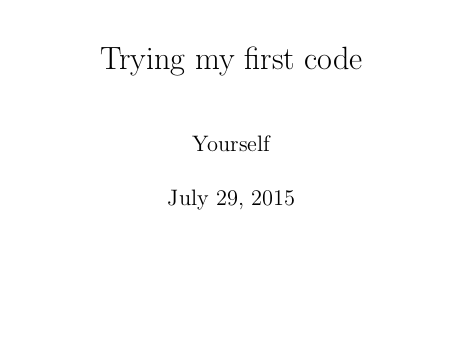
\includegraphics[scale=.5]{./lab2.png}
\caption{Image 1}
\end{figure}

\vspace{1mm}

\section{Usefull commands for LaTeX}

\begin{table} [h!]
\captionof{table}{Some basic LaTeX commands}
\begin{tabular} { |l|l| } 
\hline
 cell1 & cell2 \\
 \hline
 cell3 & cell4 \\
 \hline
 cell5 & cell6 \\
 \hline
  cell7 & cell8 \\
 \hline
\end{tabular}

\end{table}

\chapter{Working with formulas}
Here are some formulas inserted using LaTeX :

\section{Logical formulas}
In LaTeX math formulas can be written with a dollar sign. Latex also has a rich set of symbols which can be used to write the formulas. of some logical formulas are given below:
$ ( \varphi \lor \psi ) \equiv ( \psi \lor \varphi ) $
$ \neg \neg \psi \Leftrightarrow \psi $



\section{Unordered List}
\begin{itemize}
\item Item 1
\item Item 2
\item Item 3
\end{itemize}

\chapter{Other aspects of LaTeX}


\section{Images using Dia}

The below image has been drawn using Dia:

\begin{figure}[h!]

\centering
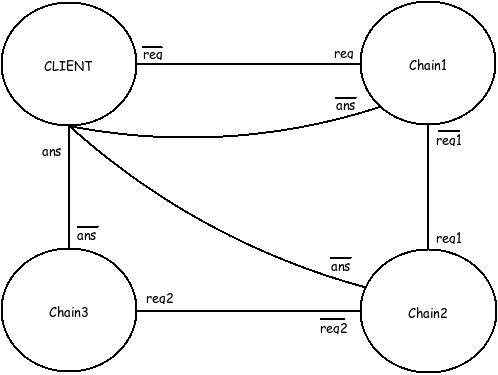
\includegraphics[scale=.7]{./lab3_dia.jpeg}
\caption{Image 2}

\end{figure}


\section{Quotes in LaTeX}
Quotes can be used easily in Latex easily using `` for left double quote and '' for right double quote. Below is the example for same.

\begin{enumerate}
 \item ``This line contains double quote.''
 \item `This line contains single quote.'
\end{enumerate}

Another quote:

\begin{figure}[h!]

\centering
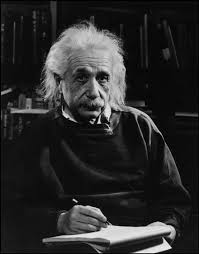
\includegraphics[scale=.7]{./ein.jpeg}

\end{figure}

"Two things are infinite: the universe and human stupidity; and I'm not sure about the universe.''


\end{document}


